\documentclass[10pt]{article}
%\usepackage{url}
%\usepackage{algorithmic}
\usepackage[margin=1in]{geometry}
\usepackage{datetime}
\usepackage[margin=2em, font=footnotesize]{caption}
\usepackage{graphicx}
\usepackage{mathpazo} % use palatino
\usepackage[scaled]{helvet} % helvetica
\usepackage{microtype}
\usepackage{amsmath}
\usepackage{subfigure}
\usepackage{listings}
\usepackage{wrapfig}
% Letterspacing macros
\newcommand{\spacecaps}[1]{\textls[200]{\MakeUppercase{#1}}}
\newcommand{\spacesc}[1]{\textls[50]{\textsc{\MakeLowercase{#1}}}}
\lstdefinestyle{myCustomMatlabStyle}{
  language=Matlab,
  stepnumber=1,
  numbersep=10pt,
  tabsize=4,
  showspaces=false,
  showstringspaces=false
}
\lstset{basicstyle=\footnotesize,style=myCustomMatlabStyle}
\title{\flushleft1.2 Ordinary Differential Equations\\ }
\date{}
\usepackage{dsfont}
\usepackage{varwidth}
\usepackage{float}

\begin{document}
\hfill\framebox{\parbox[t][5 true cm][c]{11 true cm}
{\hfil Space for project label}}
\section*{\LARGE{2.2 Collapse of a Spherical Cavitation Bubble}}

\section*{Analytic solutions for $\frac{dR}{dt}$ and $p(r,t)$}
The bubble is represented by an empty  spherical cavity of radius $R(t)$, wher $t$ is time, in an unbounded fluid which initially at rest. It may be shown that the fluid pressure $p(r,t)$ at time $t$ is given by
\begin{align}
p(r,t) &= 1+\frac{1}{r}\frac{d}{dt}(R^2\frac{dR}{dt})-\frac{R^4}{2r^4}(\frac{dR}{dt})^2\\
\intertext{An evolution equation for $R(t)$ is obtained using the boundary condition}
p(R,t) &= \frac{-2\lambda}{R}
\end{align}

\subsection*{Question 1}
To show that the equation for $R(t)$ admits a first integral, 
\begin{align}
(\frac{dR}{dt})^2 = \frac{2}{3}(\frac{1}{R^3}-1)+2\lambda(\frac{1}{R^3}-\frac{1}{R})
\end{align}
We need to show that with values from Eqn(3), we can derive the boundary condition (Eqn(2)) from Eqn(1).\\
To do this, we first differentiate (3) with respect to $t$ get
 \[\frac{d^2 R}{dt^2}=-R^{-4}+\lambda(-3R^{-4}+R^{-2})\]\\
Then, expanding equation (1) we get
\begin{flalign*}
p(r,t)&=1+\frac{1}{r}(2R(\frac{dR}{dt})^2 + R^2\frac{d^2R}{dt^2})-\frac{R^4}{2r^4}(\frac{dR}{dt})^2&\\
\intertext{Hence, setting r=R, and after simplifying we get}
p(R,t) &= 1 + \frac{3}{2}(\frac{dR}{dt})^2+R\frac{d^2R}{dt^2}&\\
\intertext{Now, by subbing in $(\frac{dR}{dt})^2$ and $\frac{d^2R}{dt^2}$ derived from Eqn(3) and simplifying, we get}
p(R,t)&= 1 + (R^{-3}-1) + 3\lambda(R^{-3}-R^{-1}) -R^{-3} + \lambda(-3R^{-3}+R^{-1}) &\\
&=\lambda(R^{-1}-3R^{-1}) \qquad \underline{= -2\lambda R^{-1}}&\\
\end{flalign*}
This matches with the given boundary condition, so $R(t)$ admits first integral Eqn(3).\\
We know that $(\frac{dR}{dt})^2\geq0$. Hence, the RHS of Eqn(3)$\geq0$. Therefore, we can solve \(\frac{2}{3}(\frac{1}{R^3}-1)+2\lambda(\frac{1}{R^3}-\frac{1}{R})=0\) to find the range that $R$ lies in.\\
The solutions are $R=1$ and $R=\frac{-(6\lambda+2)\pm\sqrt{(6\lambda+2)^2-8(6\lambda+2)}}{4}$.\\
Since $\lambda\geq0$, the latter two solutions of $R$ is always less than 0, but $R\geq0$ by assumption. Hence, $R\in[0,1]$.\\
We therefore plot $\frac{dR}{dt}$ against $R$ between 0 and 1.\\\\
The code used to plot the graph below is attached in the programs section under the title \emph{'i) q1.m'}.
\begin{figure}[h]
    \centering
    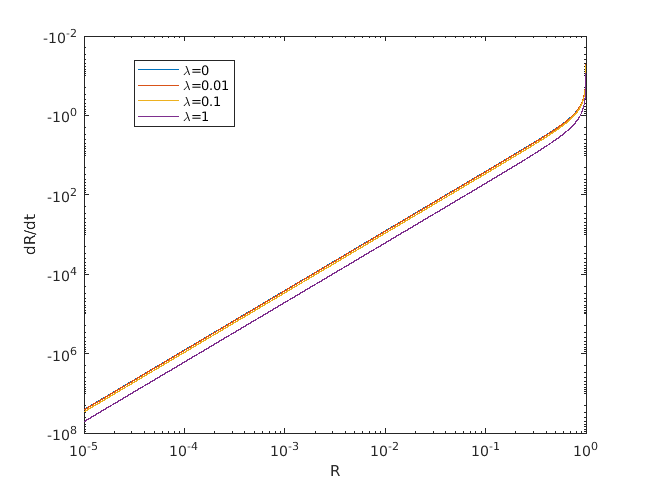
\includegraphics[width=0.55\textwidth]{q1/q1.png}
    \caption{log-log graph of $\frac{dR}{dt}$ against $R$}
\end{figure}\\
We can see that initially there is a sharp drop in $log \frac{dR}{dt}$ as $log R$ decreases from 0. But as $log R$ continues to decrease, the decrease in $log \frac{dR}{dt}$ slows down and the rate of change of decrease converges to 0, such that the curve can be described as $log(\frac{dR}{dt})= m \cdot log(R) - c$ for some constant $m$. This linear equation can also be written as $\frac{dR}{dt}=R^m\cdot 10^{-c}$.\\
We can see that $m$ is very similar regardless of the value $\lambda$ takes. However, the value of $\lambda$ does determine the value of $c$. \\
By writing $c=c_0 + \delta c$, we can also observe the difference between the curves at any given $R$ to see that the change in $\delta c$ is roughly proportional to the change in $log \lambda$, when $log\lambda >0$. But when $log\lambda <0$, $\delta c$ seems to be proportional to $10^{log \lambda}=\lambda$, converging to 0 as $log\lambda \to -\infty$.


\subsection*{Question 2}
Using results from Question 1,
\begin{flalign*}
p(r,t) &= 1+\frac{1}{r}(2R(\frac{dR}{dt})^2 + R^2\frac{d^2R}{dt^2})-\frac{R^4}{2r^4}(\frac{dR}{dt})^2&\\
&= 1 + (\frac{2R}{r}-\frac{R^4}{2r^4})(\frac{dR}{dt})^2 + \frac{R^2}{r}\frac{d^2R}{dt^2}&\\
&= 1+(\frac{2R}{r}-\frac{R^4}{2r^4})(\frac{\frac{2}{3}+2\lambda}{R^3}- \frac{2\lambda}{R} - \frac{2}{3})+\frac{R^2}{r}( \frac{\lambda}{R^2}-\frac{1+3\lambda}{R^4}) \qquad \equiv p(r,R)&\\
\end{flalign*}
We define 
\begin{align}
\alpha = \frac{1}{4}(1-4R^3)+\frac{3}{4}\lambda(1-3R^2) \qquad \text{and} \qquad \beta=1-R^3+3\lambda(1-R^2)    
\end{align}
We rearrange $p(r,R)$ to get
\begin{flalign*}
p(r,R)&= 1 + (\frac{2R}{r}-\frac{R^4}{2r^4})\times \frac{1}{3R^3}\times ((2+6\lambda)-6\lambda R^2 -2R^3) + \frac{1}{rR^2}\times (\lambda R^2 -1 -3\lambda)&\\
&=1 + \frac{1}{rR^2}(\frac{2}{3}((2+6\lambda)-6\lambda R^2 -2R^3) + \lambda R^2 -1 -3\lambda) - \frac{R}{2r^4}(\frac{2}{3}+2\lambda-2\lambda R^2 -\frac{2}{3}R^3)      &\\
&= 1+ \frac{1}{rR^2}(\frac{1}{3}(1-4R^3)+\lambda(1-3R^2))-\frac{R}{r^4}(\frac{1}{3}(1-R^3)+\lambda(1-R^2))&\\
&= 1 + \frac{1}{rR^2}\cdot\frac{4}{3}\alpha - \frac{R}{r^4}\cdot\frac{1}{3}\beta \qquad =\underline{ 1 + \frac{4\alpha}{3rR^2} - \frac{\beta R}{3r^4}}
\end{flalign*}
We know from question 1 that $\lambda\geq0$ and $R\in[0,1]$. Hence, $R^2,R^3\leq0$ implying that $\beta\geq0$ for all $R$. \\
At a time $t$, $R(t)$ becomes a constant in the equation, so $p(r,R)$ becomes a function of $r$ only. 
\begin{flalign*}
\frac{dp}{dr} &= r^{-5}(-\frac{4\alpha}{3R^2}r^3+\frac{4\beta R}{3})&\\
\Longrightarrow \qquad &\frac{1}{r^5}(-4\alpha r^3 + 4\beta R^3)=0&\\
\Longrightarrow \qquad & \underline{r=\infty} \qquad \text{or} \qquad \underline{r=(\frac{\beta}{\alpha})^{\frac{1}{3}}R} &\\
\frac{d^2p}{dr^2}&= \frac{8\alpha}{3R^2}r^{-3}-\frac{20\beta R}{3}r^{-6}
\end{flalign*}
If $\alpha<0$, then as $r=(\frac{\beta}{\alpha})^{\frac{1}{3}}R<0$ is not a solution, and $\frac{dp}{dr}>0$ for all $r$, hence $r=\infty$ is a maximum.\\
Hence, \underline{$p_{max}=p(\infty,R)=1$}.\\
If $\alpha>0$, then for sufficiently large $r$, $\frac{dp}{dr}<0$, hence $r=\infty$ is not a maximum.\\
Whereas $\frac{d^2p}{dr^2}((\frac{\beta}{\alpha})^{\frac{1}{3}}R)=R^{-5}(\frac{-12\alpha^2}{3\beta})<0$, therefore $r=(\frac{\beta}{\alpha})^{\frac{1}{3}}R$ is a maximum.\\
Therefore, \underline{$p_{max}$}$=p((\frac{\beta}{\alpha})^{\frac{1}{3}}R,R)=1+\frac{4\alpha}{3R^3}(\frac{\alpha}{\beta})^{\frac{1}{3}}+\frac{\beta R}{3}(\frac{\alpha}{\beta})^{\frac{4}{3}}R^{-4}$ \underline{=$1+R^{-3}(\frac{\alpha^4}{\beta})^{\frac{1}{3}}$}.$\qquad\qquad$(5)\\\\
The code used plot the graphs below is attached in the programs section under the title \emph{'ii) q2.m'}. To plot the graph with $\lambda=0.2,9.0$, just change the first line to the corresponding value of $\lambda$.\\ The R chosen are $0.4,0.55,0.7,0.85$ since they represent what would happen for $\alpha>0$ and $\alpha<0$.\\
\begin{figure}[h]
    \begin{minipage}[b]{0.5\linewidth}
            \centering
            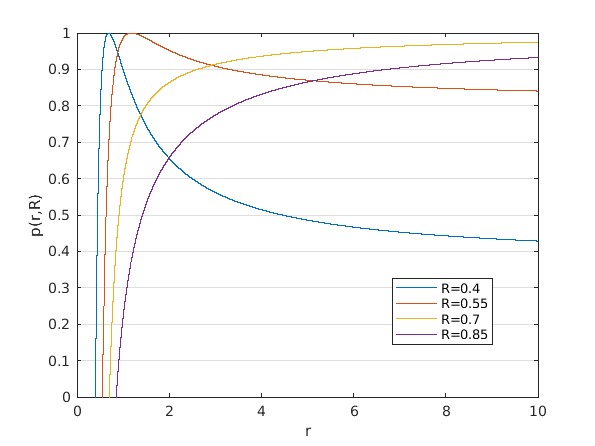
\includegraphics[width=\textwidth]{q2/q2_0.png}
            \caption{graph of p against r with $\lambda=0$}
        \end{minipage}
        \hfill
        \begin{minipage}[b]{0.5\linewidth}
            \centering
            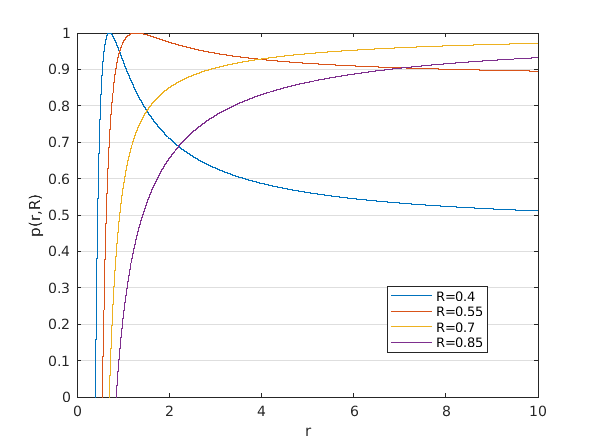
\includegraphics[width=\textwidth]{q2/q2_2.png}
            \caption{graph of p against r with $\lambda=0.2$}
        \end{minipage}
\end{figure}
\newpage
\begin{figure}[h]
    \centering
    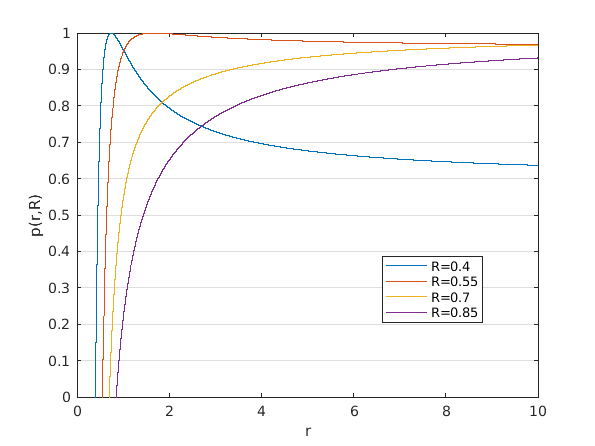
\includegraphics[width=0.5\textwidth]{q2/q2_9.png}
    \caption{graph of p against r with $\lambda=9$}
\end{figure}
\noindent Below is the values of $p_{max}$ and corresponding r.\\
\begin{tabular}{ccc}
$\lambda=0$& $\lambda=0.2$ & $\lambda=9.0$\\
\begin{tabular}{|c|c|c|}
\hline
 $R$ & $p_{max}$ & corresponding $r$\\
\hline
0.4 & 2.6959 & 0.6855 \\
0.55 & 1.2335 & 1.1837 \\
0.7 &   1 & $\infty$ \\
0.85 & 1 & $\infty$ \\
\hline
\end{tabular}
&
\begin{tabular}{|c|c|c|}
\hline
 $R$ & $p_{max}$ & corresponding $r$\\
\hline
0.4 & 3.3434 & 0.7041 \\
0.55 & 1.2502 & 1.2880 \\
0.7 &   1 & $\infty$ \\
0.85 & 1 & $\infty$ \\
\hline
\end{tabular}
&
\begin{tabular}{|c|c|c|}
\hline
 $R$ & $p_{max}$ & corresponding $r$\\
\hline
0.4 & 32.1215 & 0.7423 \\
0.55 & 2.4051 & 1.6657 \\
0.7 &   1 & $\infty$ \\
0.85 & 1 & $\infty$ \\
\hline
\end{tabular}
\end{tabular}\\\\
We observe that for all values of $R$ and $\lambda$, $p(r,R)$ increases the fastest when $r$ is small and close to the radius of the bubble $R$. The increase slows as $r$ gets larger, and $p_{min}$ is on the bubble surface.\\
We also observe that as $\lambda$ increases, then for $R$ such that its $\alpha>0$ ($R=0.4,0.55$), both its $p_{max}$ and the corresponding $r$ increases. We can also observe that relative to its normalised scale, the value of $p(r,R)$ decreases slower in $\lambda =9$ than in $\lambda=0,0.2$. And its value as $r\to\infty$ is higher as a fraction of $p_{max}$ as well.\\
And for $R=0.7,0.85$, its increase in $p(r,R)$ relative to the normalised scale slows down as $\lambda$ is increased. e.g. $p(2,0.7)\sim0.85$ when $\lambda=0$ but $p(2,0.7)\sim0.8$ when $\lambda=9$.

\bigskip\bigskip

\section*{No surface tension case}
\subsection*{Question 3}
We can define a dependable vatiable $x$, such that $x=R^{\frac{5}{2}}$,\\
and therefore,
\begin{flalign*}
\frac{dx}{dt}&=\frac{5}{2}R^{\frac{3}{2}}\frac{dR}{dt}&\\
&= -\frac{5}{2}\cdot [\frac{2}{3}(1-R^3) + 2\lambda (1-R^2)]^{\frac{1}{2}} &\\
&= -\frac{5}{2}\cdot [\frac{2}{3}(1-x^{\frac{6}{5}}) + 2\lambda (1-x^{\frac{4}{5}})]^{\frac{1}{2}}  &(6)
\end{flalign*}
Since $x\in[0,1]$ and $\lambda\geq0$, we observe $\frac{5}{2}\cdot [\frac{2}{3}(1-x^{\frac{6}{5}}) + 2\lambda (1-x^{\frac{4}{5}})]^{\frac{1}{2}}\geq0$ for all values of $\lambda,x$.\\
We also know that as $t$ increases, $x$ should get smaller to model the collapse of the bubble. This implies $\frac{dx}{dt}\leq0$. Therefore, we must take the negative root and not the positive root. Because taking the positive root would mean $\frac{dx}{dt}\geq0$, and this contradicts with a decreasing $x$. Also, taking the positive root would imply the bubble is expanding which doesn't make sense in this context.\\
Eqn (6) is non-analytic at $x=0$.  This means that the Taylor series of the solution to Eqn(6) at $x=0$ doesn't converge to the solution in some neighbourhood around $x=0$.\\
The normal benefit of using higher order methods (such as Runge-Kutta) is that the numerical solution $x_{n+1}$ we obtain from $x_n$ would be the same as the function's Taylor series expansion around $x_n$ for a higher order of terms, and hence there is a smaller local error, and our numerical solution would converge to the actual solution better than using a lower order method.\\
But as these Taylor series starts to fail to converge to the solution itself as $x\to0$, then there's no point to use a method that matches the Taylor series to a higher order, since it doesn't reduce the error to the actual solution anymore, and is slower than lower order methods.\\\\
To avoid the trivial solution $x=1$ for all $t$, we find a series solution for small time, then we can resume to use the forward Euler method.\\
We let
\begin{flalign*}
x&=\sum_{n=0}^\infty a_nt^n &\\
x(0)=1 \qquad &\Longrightarrow \qquad a_0 =1 &\\
\intertext{Then we can write $x^{\frac{6}{5}}$ as a series using binomial expansion since $|\sum_{n\geq1}x|<1$,}
x^{\frac{6}{5}} &= (1-\sum_{n\geq1} a_nt^n)^{\frac{6}{5}} &\\
&= 1+ \frac{6}{5}(\sum_{n\geq1} a_nt^n) + \frac{3}{25}\sum_{n\geq1} (a_nt^n)^2+\dots &\\
&=1 + \frac{6}{5}a_1t + (\frac{6}{5}a_2 + \frac{3}{25}a_1^2)t^2 + \mathcal{O}(t^3) &\\
\intertext{And similarly,}
x^{\frac{4}{5}} &= 1 + \frac{4}{5}a_1t + (\frac{4}{5}a_2-\frac{2}{25}a_1^2)t^2+ \mathcal{O}(t^3) &\\
\intertext{We differentiate the series expansion of $x$ to get}
\dot{x}&=\sum_{n=1}^\infty n\cdot a_n t^{n-1} &\\
\intertext{Therefore, subbing the series back into Eqn(6), we get}
(\sum_{n=1}^\infty n\cdot a_n t^{n-1})^2 &= \frac{25}{4}\cdot[\frac{2}{3}(-\frac{6}{5}a_1t - (\frac{6}{5}a_2 + \frac{3}{25}a_1^2)t^2) + 2\lambda(-\frac{4}{5}a_1t - (\frac{4}{5}a_2-\frac{2}{25}a_1^2)t^2)] + \mathcal{O}(t^3) &\\
LHS &= a_1^2 + 4a_1a_2t + (4a_2^2 +6a_1a_3)t^2 + \mathcal{O}(t^3) &\\
RHS &= \frac{25}{4}[(-\frac{4}{5}-\frac{8\lambda}{5})a_1t - ((\frac{4}{5}+\frac{8\lambda}{5})a_2+(\frac{2}{25}-\frac{4\lambda}{25})a_1^2)t^2]+\mathcal{O}(t^3) &\\
\intertext{Equating LHS and RHS, we get $a_1=0$, and therefore}
4a_2^2 &= -\frac{25}{4} (\frac{4}{5} +\frac{8\lambda}{5})a_2 &\\
a_2 &= -\frac{5}{4}(1+2\lambda)
\end{flalign*}
Therefore, \[\underline{x= 1 -\frac{5}{4}(1+2\lambda)t^2 + \mathcal{O}(t^3)} \]
In this question, $\lambda=0$, therefore for the first step in our numerical method, we let $x_1 = 1-\frac{5}{4}h^2$, where $h$ is small. And we shall proceed with Euler method now onward. This will avoid the trivial solution $x=1$.\\\\
\noindent By performing further substitution $x=sin^{5/3}\theta$, we see Eqn(6) with $\lambda=0$ becomes
\begin{flalign*}
\frac{5}{3}\dot{\theta}\cos\theta \sin^{\frac{2}{3}}\theta &= -\frac{5}{2}[\frac{2}{3}(1-\sin^2\theta)]^{\frac{1}{2}} &\\
\dot{\theta}\cos\theta\sin^{\frac{2}{3}}\theta &= -\frac{\sqrt{6}}{2}\cos\theta &\\
\dot{\theta} &= -\frac{\sqrt{6}}{2}\sin^{-\frac{2}{3}}\theta &\\
\int 1 \quad dt &= \int -\frac{2}{\sqrt{6}}\sin^{\frac{2}{3}}\theta \quad d\theta &(*)
\end{flalign*}
We know that initially at $t=0$, $R=1$; and when the bubble collapse at $t=t_c$, $R=0$.\\
Therefore, $x=1$ at $t=0$ and $x=0$ at $t=t_c$.\\
Therefore, at $t=0$, $\theta = sin^{-1}(1)=\frac{\pi}{2}$; and at $t=t_c$, $\theta=sin^{-1}(0)=0$.\\
We then sub in these as the lower and upper limit of $(*)$ to get
\[t_c = \int_{\frac{\pi}{2}}^0 -\frac{2}{\sqrt{6}}sin^{\frac{2}{3}}\theta \quad d\theta \quad = \quad \int^{\frac{\pi}{2}}_0 \frac{2}{\sqrt{6}}sin^{\frac{2}{3}}\theta \quad d\theta\]
We solve this numerically using the trapezium rule with $n=10^7$ intervals. The code used is attached in the programs section under the title \emph{'iii) q3 \textunderscore NumInt.m'}.\\
And the solution we get is \underline{$t_c = 0.91468$} (5d.p.).\\\\
We now return to solving Eqn(3) for $R(t)$ with $\lambda=0$.\\
We do this by first solve Eqn(6) numerically with forward Euler method starting from $x(h)=1-\frac{5}{4}h^2$, with step size $h=10^{-7}$. We determine $t_c$ to be the average time between $t=ih$ and $t=(i+1)h$ such that $x(ih)>0$ and $x((i+1)h)<0$. We then find $R(t)=x(t)^{\frac{2}{5}}$, and plot it against $t$ from $0$ to $t_c$.\\
We can then also find $p_{max}(t)$ and plot it against $t$ using a semi log scale.\\
The code used to do this is attached in the programs section under the title \emph{'iv) q3\textunderscore main.m'}.\\
Using this method, we found $t_c=0.91468225$. This agrees with the value found via numerically integrating.
\begin{figure}[ht]
    \begin{minipage}[b]{0.48\linewidth}
            \centering
            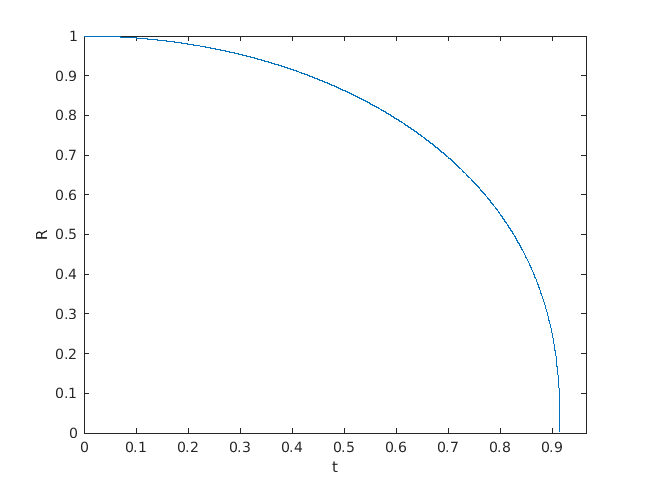
\includegraphics[width=\textwidth]{q3/q3_R.png}
            \caption{graph of $R(t)$ against $t$ with $\lambda=0$}
        \end{minipage}
        \hfill
        \begin{minipage}[b]{0.48\linewidth}
            \centering
            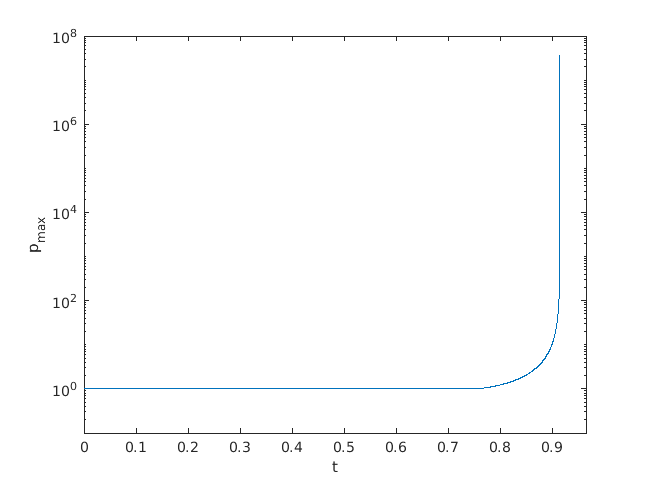
\includegraphics[width=\textwidth]{q3/q3_p2.png}
            \caption{graph of $p_{max}$ against $t$ with $\lambda=0$}
        \end{minipage}
\end{figure}\\
We can see that initially $R(t)$ decreases slowly, but as $t$ increases, and $R(t)$ gets smaller, the magnitude of its rate of decrease gets larger and larger.\\ Correspondingly, $p_{max}=1$ for the initial stage of decrease where $\alpha<0$ and $p_{max}$ is occuring at $r=\infty$, but as $R$ decreases, $\alpha$ increases past 0, and $p_{max}$ increases proportionally to $R^{-7}$ (since $\alpha\sim R^{-3}, \beta\sim1$ as $R\to0$). The position $r$ of $p_{max}(t)$ also moves towards $R(t)$.\\\\
We proceed to consider the numerical accuracy of $R(t)$ in this question.\\
We've picked our first step to be at $t=10^{-7}$ such that it has a small error to the actual $x$ ($\sim\mathcal{O}(h^3)$).\\
We know Euler method has local truncation error of $\frac{x''}{2}h^2$. We can differentiate Eqn(6) wrt. $t$ again to find that \[x''=\frac{-5\cdot1\cdot-2\cdot6}{2\cdot2\cdot3\cdot5}x^{\frac{1}{5}}x'(\frac{2}{3}(1-x^{\frac{6}{5}})^{-\frac{1}{2}}\]
\[x''=-\frac{5}{2}x^{\frac{1}{5}}\]
This shows that the magnitude of the local truncation error of each step is strictly smaller than $\frac{5}{4}h^2=\frac{5}{4}\cdot 10^{-14}$, since we started slight from a suitable non-zero time, and the local truncation error tends to 0 as $x$ tends to 0.\\

\section*{With surface tension case}
\subsection*{Question 4}
From Question 3, we know the following
\[\frac{dx}{dt}= -\frac{5}{2}\cdot [\frac{2}{3}(1-x^{\frac{6}{5}}) + 2\lambda (1-x^{\frac{4}{5}})]^{\frac{1}{2}}\]
We take the first step in our numerical methods to be $x_1 = 1-\frac{5}{4}(1+2\lambda)h^2$, where $h$ is small. And proceed with forward Euler.
We choose a set of $\lambda$ to do this. And the set we picked is [0.01,0.1,0.5,1,10,100,1000].\\
We plotted the graphs of $R(t)$ against $t$ and $p_{max}(t)$ against $t$ for these values of $\lambda$. The code to do this is attached in the programs section under the titles \emph{'v) q4\textunderscore R.m'} and \emph{'vi) q4\textunderscore Pmax.m'} respectively.\\
\begin{figure}[ht]
    \begin{minipage}[b]{0.55\linewidth}
            \centering
            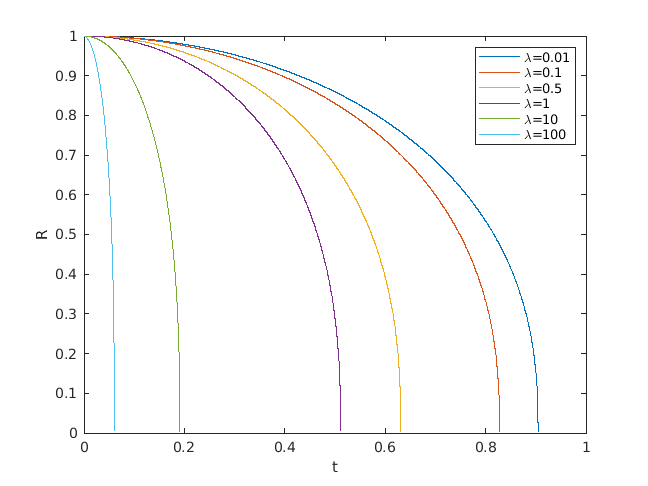
\includegraphics[width=\textwidth]{q4/q4_R.png}
            \caption{graph of $R(t)$ against $t$}
        \end{minipage}
        \hfill
        \begin{minipage}[b]{0.55\linewidth}
            \centering
            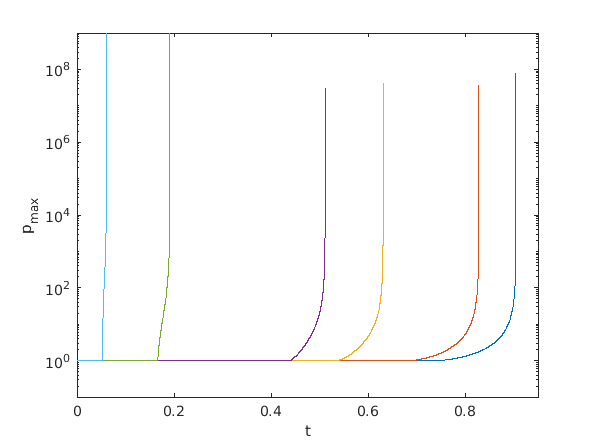
\includegraphics[width=\textwidth]{q4/q4_Pmax.png}
            \caption{graph of $p_{max}$ against $t$}
        \end{minipage}
\end{figure}\\
These two graphs shares legend.\\
\begin{figure}[ht]
    \centering
    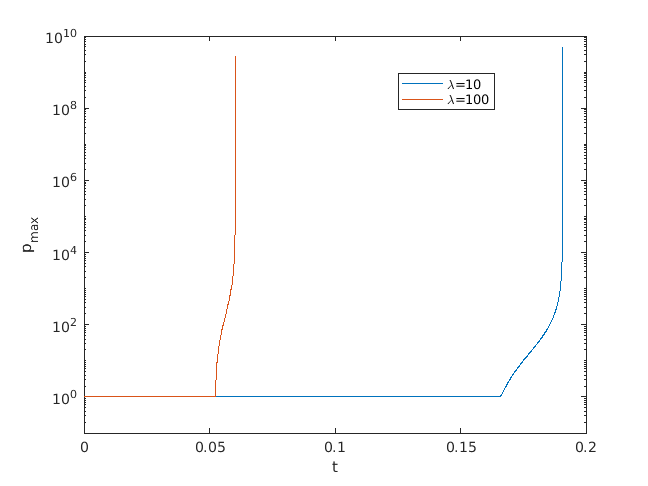
\includegraphics[width=0.48\textwidth]{q4/q4_P_large_lambda.png}
    \caption{graph of $p_{max}$ against $t$ for large $\lambda$}
\end{figure}\\
\noindent We see that as $\lambda$ increases, the time it takes for the bubble to collapse decreases, and the rate of change in $t_c$ also decreases. This shows that the stronger the surface tension is, the shorter time the bubble can exist.\\
This is also shown in the $p_{max}(t)$ graph. We can see that the value of $t$ where $R(t)$ gets small enough such that $\alpha>0$ (call $t_\alpha$) is getting larger as a proportion of $t_c$ as $\lambda$ gets larger ($\frac{t_\alpha}{t_c}\to1$); and the rise in $p_{max}$ after such $t_\alpha$, is getting steeper as $\lambda$ increases. The increase is exponential and the rate of increase also gets larger exponentially as $t\to t_c$.\\
For larger values of $\lambda$ (e.g. see graph below), we can see that the gradient is consistent for $t$ just bigger than $t_\alpha$, but then as $t\to t_c$, the gradient increases exponentially. \\
This corresponds the rapid collapse of bubble. And it means the bubble will physically release more energy when collapsed.\\\\
Mathematically, we can perform change of variable $x=sin^{\frac{5}{3}}\theta$ again to Eqn(6). We get
\begin{flalign*}
\frac{5}{3}\dot{\theta}\cos\theta \sin^{\frac{2}{3}}\theta &= -\frac{5}{2}[\frac{2}{3}(1-\sin^2\theta)+2\lambda(1-\sin^{\frac{4}{3}}\theta)]^{\frac{1}{2}} &\\
\dot{\theta}&=\frac{-3}{2}[\frac{2}{3}\sin^{\frac{-4}{3}}\theta+\frac{2\lambda(\sin^{\frac{-4}{3}}\theta-1)}{\cos^2\theta}]^{\frac{1}{2}} &\\
\int^{t_c}_0 1\quad dt &= \int^{\frac{\pi}{2}}_0 \frac{d\theta}{\frac{3}{2}[\frac{2}{3}\sin^{\frac{-4}{3}}\theta+\frac{2\lambda(\sin^{\frac{-4}{3}}\theta-1)}{\cos^2\theta}]^{\frac{1}{2}}}
\end{flalign*}
We observe that for $\lambda$ sufficiently large,
\[\frac{2}{3}\sin^{\frac{-4}{3}}\theta+\frac{2\lambda(\sin^{\frac{-4}{3}}\theta-1)}{\cos^2\theta}\sim\frac{2\lambda(\sin^{\frac{-4}{3}}\theta-1)}{\cos^2\theta}\]
Hence 
\[t_c \sim \int^{\frac{\pi}{2}}_0 \frac{d\theta}{\frac{3}{2}[\frac{2\lambda(\sin^{\frac{-4}{3}}\theta-1)}{\cos^2\theta}]^{\frac{1}{2}}}\]
\[ = \frac{1}{\sqrt{\lambda}} \int^{\frac{\pi}{2}}_0 \frac{d\theta}{\frac{3}{2}[\frac{2(\sin^{\frac{-4}{3}}\theta-1)}{\cos^2\theta}]^{\frac{1}{2}}} \propto \frac{1}{\sqrt{\lambda}}
\]
Hence, as $\lambda\to\infty$, \underline{$t_c\propto \frac{1}{\sqrt{\lambda}}$}.\\
As for $\lambda<<1$, for any fixed $\theta$,
\[\frac{2\lambda(\sin^{\frac{-4}{3}}\theta-1)}{\cos^2\theta}\to0\]
And hence $t_c(\lambda)\to t_c(0)=0.91468$.\\

\subsection*{Question 5}
This model has several physical limitations. \\
a)\quad One is that in real life, bubbles form in fluid by trapping vapour or other gases, but this model assumes that the bubbles are empty cavities. And this has 2 impact:\\
1. the bubble would 'pop' at some $R$ such that $R>0$, whereas in this model we assumed the bubble collapse to $R=0$.\\
2. This will change the boundary conditions of $p(r,t)$ (Eqn 2) and hence changing our equation for $R(t)$ and $p_{max}(t)$.\vspace{0.3cm}\\
b) Even if the bubble is empty, the pressure will tends to $\infty$ as $R$ continues to decrease to 0. But the material of the bubble surface might not be able to maintain itself as this pressure continues to increase and hence the bubble can only collapse to some non-negative $R_c$.\vspace{0.2cm}\\
c)\quad Another limitation is that we have assumed that the pressure at large distance is a constant and the pressure is spatially symmetric (depends only on $r$ and $t$). However, this is often not the case, since bubbles are often formed near an object which means the pressure is different at large distance depending on the direction, and hence there is no symmetry of pressure at large distance.\\\\
To allow for bubbles in a liquid that are not empty but contain small amounts of vapour or other gas. We must consider the pressure inside the bubble, which is no longer 0 as in the case where the bubble is an empty cavity.\\
Assuming the vapour is an ideal gas, then by Boyle's law, the pressure inside is inversely proportional to the volume, i.e. \[p_{in}\propto\frac{1}{V}\]
Assume the bubble remains spherical, the volume inside the bubble is $\frac{4}{3}\pi R^3$, and at $t=0$, $V_0=\frac{4}{3}\pi$. \\
The equation for $p(r,t)$ where $r>R$ (Eqn(1)) is unchanged. \\
However, to balance the force on the bubble surface, we do need to change the boundary condition (Eqn(2)) to 
\[p(R,t)-p_{in}(R,t)=-\frac{2\lambda}{R}\]
Therefore, we need a reasonable estimate for $p_{in}(R=1)$.\\
Once we know that, then $p_{in}(R)=\frac{\frac{4}{3}\pi\cdot p_{in}(R=1) }{V}$, and the boundary condition above becomes
\[p(R,t)=\frac{\frac{4}{3}\pi\cdot p_{in}(R=1) }{V}-\frac{2\lambda}{R}\]


\newpage
\section*{Programs}
\subsection*{i) q1.m}
\lstdefinestyle{myCustomMatlabStyle}{
  language=Matlab,
  stepnumber=1,
  numbersep=10pt,
  tabsize=4,
  showspaces=false,
  showstringspaces=false
}
\lstset{basicstyle=\footnotesize,style=myCustomMatlabStyle}
\begin{lstlisting}
lambda = [0.0,0.1,1.0,10.0,100.0];     
R = logspace(-4,0,10000);       % log distributed points of R for plotting
dR_dt = zeros(1,numel(R));
% for loop used to plot the individual curves
for i = 1:numel(lambda)
    for j = 1:numel(R)
        dR_dt(j) = -sqrt(2/3*((1/R(j)^3)-1) +2*lambda(i)*(1/R(j)^3-1/R(j)));
    end
    plots(i) = loglog(R,dR_dt,"DisplayName",['lambda=' num2str(lambda(i))]);
    hold on
end
hold off
legend(plots)
xlabel('R'), ylabel('dR/dt')
\end{lstlisting}

\vspace{2.0cm}
\subsection*{ii) q2.m}
\lstdefinestyle{myCustomMatlabStyle}{
  language=Matlab,
  stepnumber=1,
  numbersep=10pt,
  tabsize=4,
  showspaces=false,
  showstringspaces=false
}
\lstset{basicstyle=\footnotesize,style=myCustomMatlabStyle}
\begin{lstlisting}
lambda = 0.2;
R_range = [0.4,0.55,0.7,0.85];        % choice of R
for i = 1:numel(R_range)
    R = R_range(i);     %setting value of R
    alpha = (1/4)*(1-4*R^3)+(3/4)*lambda*(1-3*R^2);
    beta = 1-R^3 + 3*lambda*(1-R^2);
% used to analytically calculate max pressure and the corresponding r
    if alpha > 0
        r_max=((beta/alpha)^(1/3))*R;
        p_max = 1 + R^(-3)*(alpha^4/beta)^(1/3);
    else
        p_max = 1;
        r_max = inf;
    end
    disp([i,r_max,p_max])
% plotting between r=0.5 and 3    
    r = linspace(R_range(i),10,10^6);        % r>R
    results = zeros(1,numel(r)+1);
    for j = 1:(numel(r))
        results(j) = 1 + 4*alpha/(3*r(j)*R^2) - beta*R/(3*r(j)^4);
    end
% below is done to avoid the situation where p_max is not 1 in the range of the plot
    results(numel(r)+1) = 1;        
% normalise the results s.t. p_max-p_min =1 
    normalised_results = normalize(results,'range');    
    plot(r,normalised_results(1:numel(r)), ...
        'DisplayName',['R=' num2str(R_range(i))])
    hold on 
end
set(gca,'YGrid',"on")
xlabel('r'),ylabel('p(r,R)')
hold off
legend
\end{lstlisting}
\newpage
\subsection*{iii) q3\textunderscore NumInt.m}
\lstdefinestyle{myCustomMatlabStyle}{
  language=Matlab,
  stepnumber=1,
  numbersep=10pt,
  tabsize=4,
  showspaces=false,
  showstringspaces=false
}
\lstset{basicstyle=\footnotesize,style=myCustomMatlabStyle}
\begin{lstlisting}
% numerical integration using trapezium rule
format long
f = @(x) (2/sqrt(6)).*(sin(x).^(2/3));
a = 0;
b = pi/2;
n = 10^7;       % number of intervals
h = (b-a)/n;
sum_temp = f(a)+f(b);
for i = 1:n
    sum_temp = sum_temp + 2*f(a+h*i);
end
I = (h/2)* sum_temp;
disp(I)
\end{lstlisting}
\vspace{2.0cm}
\subsection*{iv) q3\textunderscore main.m}
\lstdefinestyle{myCustomMatlabStyle}{
  language=Matlab,
  stepnumber=1,
  numbersep=10pt,
  tabsize=4,
  showspaces=false,
  showstringspaces=false
}
\lstset{basicstyle=\footnotesize,style=myCustomMatlabStyle}
\begin{lstlisting}
format long
h = 10^(-7);
n = 1/h;
lambda = 0;
f = @(x,t) (-5/2)*sqrt((2/3)*(1-x^(6/5)));    % formula for dx/dt, lambda=0

X(1) = 1;     % val x(0)
X(2) = 1 - (5/4)*h^2;   % val x(h)

i = 2;      % corresponding to x((i-1)*h)
while X(i) > 0
    X(i+1) = X(i) + h * f(X(i),i*h);        % forward euler
    i = i+1;
end
t_c = (i-1/2)*h;    % t average between 1st neg. and last pos. val of x
disp(t_c)

t_range = 0:h:(i-2)*h;
R = X.^(2/5);
% plotting R against t
figure(1)
plot(t_range,R(1:i-1))
xlim([0,t_c+0.05]),ylim([0,1]),xlabel('t'),ylabel('R')
% finding p_max(t)
for j = 1:i-1
    alpha = (1/4)*(1-4*R(j)^3)+(3/4)*lambda*(1-3*R(j)^2);
    beta = 1-R(j)^3 + 3*lambda*(1-R(j)^2);
    if alpha > 0
        p_max(j) = 1 + R(j)^(-3)*(alpha^4/beta)^(1/3);
    else
        p_max(j) = 1;
    end
end
% plotting p_max against t
figure(2)
plot(t_range,p_max)
set(gca, 'YScale', 'log')
xlim([0,t_c+0.05]),xlabel('t'),ylabel('p_{max}')
\end{lstlisting}
\newpage
\subsection*{v) q4\textunderscore R.m}
\lstdefinestyle{myCustomMatlabStyle}{
  language=Matlab,
  stepnumber=1,
  numbersep=10pt,
  tabsize=4,
  showspaces=false,
  showstringspaces=false
}
\lstset{basicstyle=\footnotesize,style=myCustomMatlabStyle}
\begin{lstlisting}
format long
lambda = [0.01,0.1,0.5,1,10,100];
for k = 1:numel(lambda)
    if lambda(k) > 1        % for better accuracy with large lambda
        h = 10^(-8);
        n = 1/h;
    else
        h = 10^(-7);
        n = 1/h;
    end
    f = @(x,t) (-5/2)*sqrt((2/3)*(1-x^(6/5))+2*lambda(k)*(1-x^(4/5)));    % formula for dx/dt, lambda=0
    X(1) = 1;     % val x(0)
    X(2) = 1 - (5/4)*h*(1+2*lambda(k))^2;   % val x(h)
    
    i = 2;      % corresponding to x((i-1)*h)
    while X(i) > 0
        X(i+1) = X(i) + h * f(X(i),i*h);        % forward euler
        i = i+1;
    end
    t_c = (i-1/2)*h;    % t average between 1st neg. and last pos. val of x
    disp(t_c)
    
    t_range = 0:h:(i-2)*h;
    R = X.^(2/5);
% plotting R against t
    figure(1)
    plot(t_range,R(1:i-1),"DisplayName",['\lambda=', num2str(lambda(k))])
    hold on
    xlabel('t'),ylabel('R')
    
    clear X i h n
end
hold off
legend
\end{lstlisting}
\vspace{2.0cm}
\subsection*{vi) q4\textunderscore Pmax.m}
\lstdefinestyle{myCustomMatlabStyle}{
  language=Matlab,
  stepnumber=1,
  numbersep=10pt,
  tabsize=4,
  showspaces=false,
  showstringspaces=false
}
\lstset{basicstyle=\footnotesize,style=myCustomMatlabStyle}
\begin{lstlisting}
format long
lambda = [0.01,0.1,0.5,1,10,100];
for k = 1:numel(lambda)
    if lambda(k) > 1
        h = 10^(-8);
        n = 1/h;
    else
        h = 10^(-7);
        n = 1/h;
    end
    f = @(x,t) (-5/2)*sqrt((2/3)*(1-x^(6/5))+2*lambda(k)*(1-x^(4/5)));    % formula for dx/dt, lambda=0
    X(1) = 1;     % val x(0)
    X(2) = 1 - (5/4)*h*(1+2*lambda(k))^2;   % val x(h)
    
    i = 2;      % corresponding to x((i-1)*h)
    while X(i) > 0
        X(i+1) = X(i) + h * f(X(i),i*h);        % forward euler
        i = i+1;
    end
    t_c = (i-1/2)*h;    % t average between 1st neg. and last pos. val of x
    disp(t_c)
    
    t_range = 0:h:(i-2)*h;
    R = X.^(2/5);
    % finding p_max(t)
    for j = 1:i-1
        alpha = (1/4)*(1-4*R(j)^3)+(3/4)*lambda(k)*(1-3*R(j)^2);
        beta = 1-R(j)^3 + 3*lambda(k)*(1-R(j)^2);
        if alpha > 0
            p_max(j) = 1 + R(j)^(-3)*(alpha^4/beta)^(1/3);
        else
            p_max(j) = 1;
        end
    end
% plotting p_max against t
    plot(t_range,p_max,"DisplayName",['\lambda=', num2str(lambda(k))])
    set(gca, 'YScale', 'log')
    xlim([0,0.95]),xlabel('t'),ylabel('p_{max}'),ylim([10^(-1),10^9])
    hold on
    clear X i h n p_max
end
hold off
\end{lstlisting}

\end{document}
